\documentclass{ltjsarticle}
\usepackage{docmute} 
\usepackage{myStyle} 

\begin{document}

\chapter{確率分布とデータの関係}
\label{chapter24}
検定では平均因果効果を検証するため，平均値や(不偏)分散などの標本統計量がどのような確率分布に従うかを参照し，結果を判定するという使い方を行なってきました。検定はこのように，母数を推定する方法に，結果を判定するロジックが組み合わさったものなのでした。この時の母数の推定方法は，標本平均や不偏分散を推定値とする方法で，モーメント法とよばれるものです。これに対し，モデルである確率分布をデータに最も近しい形に調節することで，そのパラメータを推定値とする方法があります。ここではこの方法，最尤推定法とその根幹にある尤度という考え方を解説します。
\section{確率モデルによる推論}
もう一度，後期のテーマである統計的推論の基本を振り返ってみましょう。

私たちは，手元にあるデータの状態を記述するだけでなく，これを使って「推論」をしたいわけです。覚えていますか？手元のデータ(標本)において，群間に差があるかどうか！なんて考えなくても「そりゃあるでしょ」となります。微細な差でも差は差ですから，それは違いありません。問題は，手元の標本の特徴を使って，「だから人間は・・・」などと大きな主語のことを言おうとすると，ちょっと待て待て，となるわけです\footnote{でも人間は，自分の経験を使っていろいろ言いたい生き物です。政治家だって，タレントだって，それでいろいろ失敗してますよね。でも例えば「どうして男性は浮気するのか！」と怒っている人に「サンプルサイズが少なすぎる。それでは妥当な推論ができないから，せめて20人以上と交際してから言え」なんていうと逆ギレされるかしらけられるかのどちらかです。統計家は辛いよ。}。たまたま標本の数字がそうだっただけじゃないか，というわけですね。ここでいう「大きな主語のことを言おうとする」，というのが統計的推論という話なので，そもそも雲を掴むようなというか，無理難題に挑戦しているというのが大前提，何も確定的に言えないんじゃないかとさえ思えてきます。

そこをぐっと堪えて，仮に，仮にですよ？仮に母集団の数字が正規分布に従うと仮定できるのであれば，そこから原理的に標本統計量の特徴が導かれますから，それを使って推論しようよ，という話をしてきたのでした。

さて，今回までの話は母集団が正規分布するなら，標本統計量がある程度の幅を持った正規分布に従うので，標本平均や標本分散を使って推定しましょう，というアプローチをとってきました。平均値や分散など，標本の特徴そのものから母数を推定してきましたが，今回からお話しするのは少し異なるアプローチです。それは，\keyterm{確率モデル}の考え方の入り口であり，これを知ることで線形モデルの表現がより豊かになっていきます。

\section{確率関数と尤度}
確率とデータの関係について，改めて考えてみましょう。

確率分布の形がわかっていて，パラメータもわかっていたとします。例えば$\theta=0.5$のベルヌーイ分布だとか，平均値$\mu=5$，標準偏差$\sigma=1$の正規分布，といった具合に。そうすると，そこからデータがどう出てくるかを考えることができます。ベルヌーイ分布の例がわかりやすいので，それで考えてみましょう。とあるコインの表が出るか裏が出るかが，$\theta=0.5$のベルヌーイ分布に従う，というのがわかっていたら，きっと表(1)と裏(0)が半々で出てくるだろうな，と思えるわけです。$\theta=0.7$であれば，こりゃ表がよく出てくるだろうな，といったことがわかります。

ただ私たちが，確率的なことを考える時というのはもっぱら逆です。表，表，裏，表，表・・・とどうも表がたくさん出てくるという現実があり，「これのパラメータは$\theta=0.5$ではないのではないか(半々じゃない，イカサマコインだ)」といったように，実現値が既知でパラメータが未知な状況です。研究をしている時も，手元にデータがあって，パラメータがわからないわけです。これまで推論してきた母平均，母分散というのもパラメータですが，そこから得られたと思しきデータを使って推論してきたのでした。

もう少し考えを深めてみましょう。ベルヌーイ分布は次のような確率分布です。
$$ p(k) = \theta^k (1-\theta)^{1-k}$$
ここで$k$は1か0のどちらかの数字をとります。表が出る確率$p(1)$は，$\theta^1 ( 1-\theta)^0 = \theta$になり\footnote{ある数字の0乗は1になる，というのが累乗の計算のルールです。}，裏が出る確率は$p(0) = \theta^0(1-\theta)^k=(1-\theta)$になる，ということを数式で書くとこうなるのです。試しに$\theta=0.7$とすると，表が出る確率が$0.7$で裏が出る確率が$0.3$になっていますね。わかりやすい。

ここで$\theta=0.7$，のようにパラメータがわかっている状況は普通とは逆なのですから，パラメータがわからない未知のまま($\theta$の記号のまま)考えを進めたいと思います。もしコインが表，表と2回続けて表が出るとすると，その確率は$\theta \times \theta = \theta^2$です。3回続けて出たら$\theta^3$，表，表，裏，裏，表なら$\theta^3\times (1-\theta)^2$，と文字を使って表現できます。ここで$\theta$は0から1の間を取る数字ですから，横軸に$\theta$をとり，，縦軸に$y=\theta^3\times (1-\theta)^2$として関数のグラフを書くことができますね。これを書いたのが図\ref{fig::24_01}です。
\begin{figure}[ht]
    \centering
    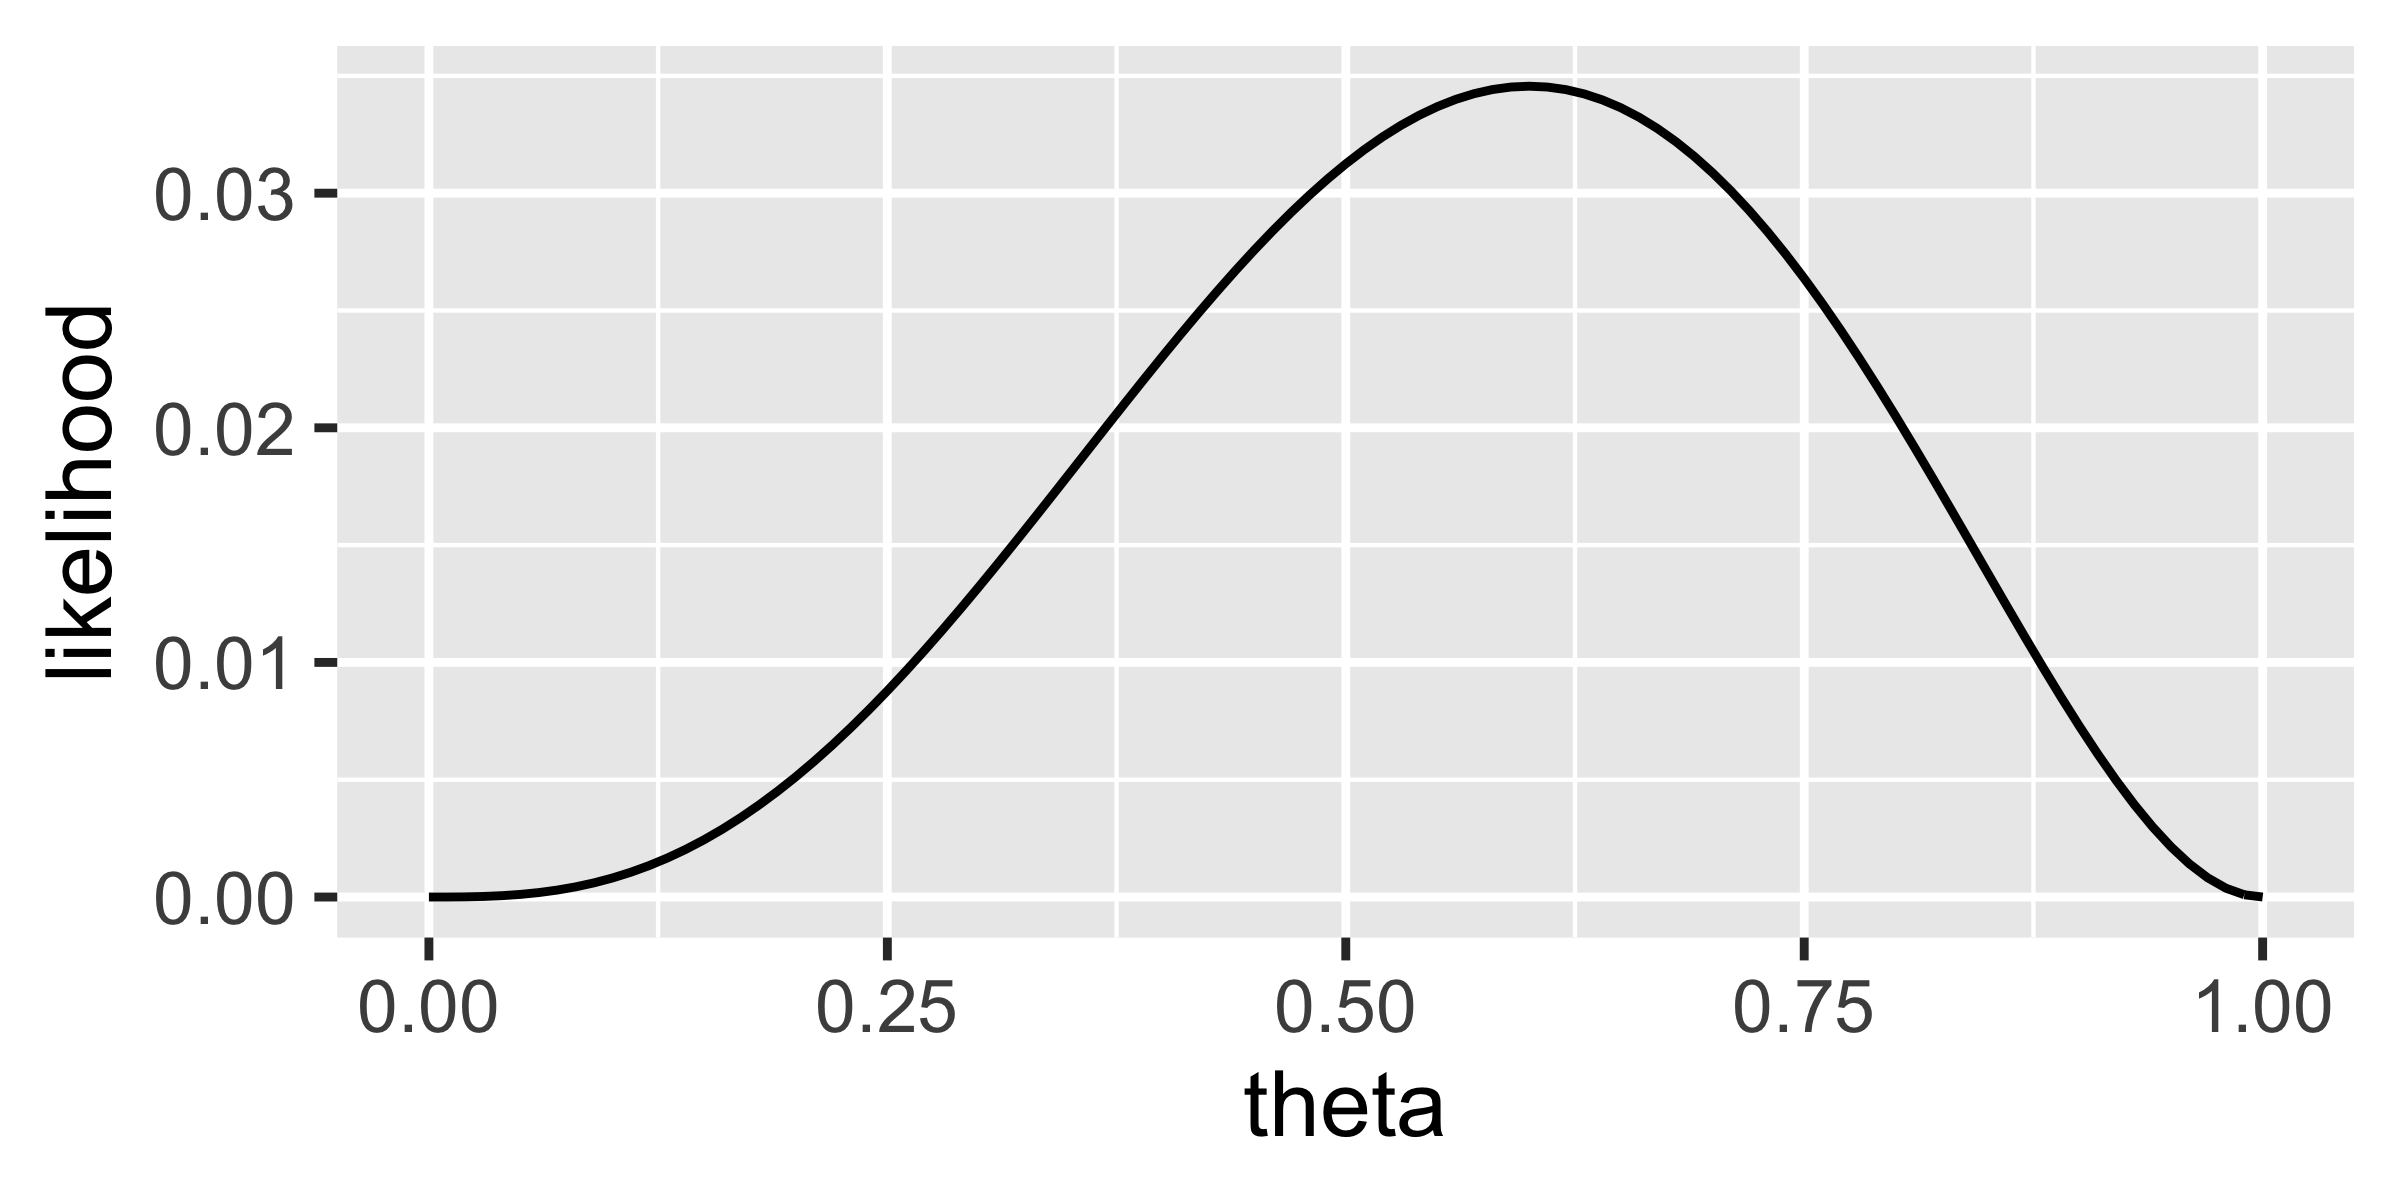
\includegraphics[keepaspectratio,width=6cm]{images/text24/Rplot24_01.png}
    \caption{「表，表，裏，裏，表」と出たコインのパラメータの関数}
    \label{fig::24_01}
\end{figure}
これはパラメータがどのあたりにありそうか，という情報を持ったグラフになっています。このように，データが既知でパラメータが未知のとき，パラメータの関数のことを\keyterm{尤度関数}といい，このグラフの縦軸$y$のことを\keyterm{尤度}likelihood と言います\footnote{ゆうど，と読みます。犬度(いぬど)ではありません。尤度の尤は，「もっとも」と読み「尤もらしい」といったりします。}

尤度関数は確率関数と形Formは同じですが，考える向きを逆にしたものだと言えます。つまり，
\begin{itemize}
    \item 確率関数；パラメータがわかっている$\to$実現値がどのように出てくるかを表現
    \item 尤度関数；実現値がわかっている$\to$パラメータがどのあたりならこのデータが得られそうかを表現
\end{itemize}
という関係にある，というわけです。

\section{最尤推定}
さてこの尤度関数，横軸が$\theta$ですから，いろいろな$\theta$の時にこのデータが得られる可能性はどれぐらいありそうか，というグラフだといえます。そうするとこの山のピーク，ここでは$\theta=0.6$なのですが，これが「このデータから考えられる\underline{最もありえそうな}パラメータの値」ということになります。尤度が最大になるところをそのパラメータの推定値とする，という意味で，この推定値を\keyterm{最尤推定値}といい，この方法でパラメータのことを推定する方法を\keyterm{最尤法}Maximum Likelihood methodといいます(さいゆう推定，と読みます。略してML法とかかれることも)。

5回中3回表が出たから，パラメータは$0.6$なのは当たり前じゃないか，と思ったかもしれません。それは標本平均を使って推定した，ということですが，同じ現象・データなので推定値が同じになるのはまあ当然のことです。答えは同じなのですが，その答えを出した筋道が違う，ということに注目してください。

最尤法は，関数の最大値を求めることによって最尤推定値を算出します。「関数の最大値を求める」という方法は，具体的には微分をつかって極限を求めることになります。微分について，高校数学で学んできたことを思い出して欲しいのですが，要するに「関数の傾きがフラットになる(傾き$0$)ところがその関数の最大値，あるいは最小値になっている」という性質から，傾きの関数を求めてそれがどこなのか，を突き止める方法であり，まさに今回のようにピークを求めるにはもってこいのツールだったわけです\footnote{高校までの数学は，こうした目的を先に教えておいてくれたらイメージしやすいのですが，先に概念や計算方法だけ教わるので苦手意識を持っている人もいるかもしれません。完成図を見ずにパズルのピースだけ渡されても，興味は持ちにくいかもしれませんが，幸い目的を持って学び始めると，いつ・どこから始めても必ず道がつながっているので，いつでも学び直すと良いでしょう。}
\footnote{今回，この関数を微分すると，
\begin{eqnarray*}
    y &=& \theta^3(1-\theta)^2 \\
    & =& \theta^3(1-2\theta+\theta^2)\\
    &=& \theta^3 - 2\theta^4 + \theta^5 \mbox{より}\\
    y' &=& 5\theta^4 - 8\theta^3 + 3\theta^2\\
    &=& \theta^2(5\theta^2-8\theta+3)
\end{eqnarray*}
ここで$y'=0$とおいて極値を求めると
\begin{eqnarray*}
    (5\theta^2-8\theta+3) &=& (\theta -1)(5\theta -3)
\end{eqnarray*}
より，$0< \theta < 1$の範囲では$\theta=3/5=0.6$が極大ということになります。
}。

細かい数式はともかく，要するに関数のピークは最も尤もらしい，つまりこのデータが出てくる確率を最大にする値としてパラメータを推定できるということです。

ここで一点，注意を促しておきます。尤度関数は，確率分布関数の未知数と既知数を取り換えただけのものです。確率分布関数は，確率の出目(実現値)に対応する確率の一覧を数式で表現したものだったことを思い出してください。また，確率とは非負で，その総和が1.0になるような数字なのでした。ここで図\ref{fig::24_01}を見ていると，これもなんだか確率分布のように見えたりもしますが，実はこれは確率分布ではありません。というのも，この関数の面積が1.0にならないからです。

簡単な例で解説しましょう。コイントスを2回連続でやることを考えてみたいと思います。この時何回表が出てくるかは，0回(裏・裏)，1回(裏・表，表・裏),2回(表・表)のいずれかです。

\begin{table}[ht]
    \centering
    \caption{コインを二回トスします。} 
    \begin{tabular}{rrrrr}
      \hline
    $\theta$  & 0回 & 1回 & 2回 & 合計 \\
    \hline
    0.00 & 1.00 & 0.00 & 0.00 & 1.00\\
    0.25 & 0.5625 & 0.375 & 0.0625 & 1.00\\
    0.50 & 0.25 & 0.50 & 0.25 & 1.00\\
    0.75 & 0.0625 & 0.375 & 0.5625 & 1.00\\
    1.00 & 0.00 & 0.00 & 1.00 & 1.00\\
    \hline
    合計 & 1.9525 & 1.175 & 1.9525 &  \\
    \hline
    \end{tabular}
      \label{tbl::24_01}
\end{table}

表\ref{tbl::24_01}をみてください。これはコインを2回トスして，何回表が出たかについて，$\theta$をいろいろに変えて計算してみた表です。例えば$\theta=0.0$であれば，完全に裏しか出ないコインなのですから，0回の確率が100\%で，1回，2回出る可能性は0\%です。この行方向の総和は$1.00$になっています。どの行についても，行の総和は$1.00=100\%$で，$\theta$が決まっているとしたらデータがどうなるかの確率は計算できるわけです。

一方，2回コイントスして，1回も表が出なかったという事実が先にあったとします。表\ref{tbl::24_01}でいうところの0列，縦方向にみるのですね。$\theta$は0から1のどこかにあるのですが，$0.00,0.25,0.50,0.75,1.00$の4パターンだけピックアップしてみてみても，その総和は1.00を超えています。これを見ると，1回も表が出ないパターンというのは，$\theta=1.0$であるはずがなく，$\theta=0.75$のような高い確率でもなさそう，$0.5,0.25$とパラメータが小さくなるに従って「そうなりそうな度合い」は高くなっていき，$\theta=0.00$であるというのが一番あり得そうではありますが，$\theta=0.00$の確率が高い，とは言えないのです。列の総和が1.00にならないから，これ(尤度)は確率じゃないからです。尤度は確率ではないのです\footnote{この表を使った説明の仕方は，私がみてきた「尤度は確率じゃない」の説明の中で最もわかりやすいもので，\citet{lambert2018student}にあった説明の仕方です。ここではその数字を少し改変して紹介しました。}。

尤度が最も高い，というのはそうなる可能性が最も高いわけですが，この数字は確率じゃない--ちょっと面倒な感じですが，言葉を正確にいうとこうなりますので，ご容赦ください。あくまでも，もっともらしさ，それっぽさが最大になるように推定値を定めるというのが最尤推定の正しい説明になります。
\section{対数と尤度}
ところで，尤度の最大値を求める計算は，微分を使うのでちょっと面倒だな，と思うかもしれませんが，具体的な数値にしてしまえばそれほど大変ではありません。例えば先ほどの例，ベルヌーイ試行(コイントス)で表が3回，裏が2回でた，という場合ですが，$\theta=0.3$であれば，
$$ 0.3^3 \times (1-0.3)^2 = 0.3 \times 0.3 \times 0.3 \times 0.7 \times 0.7 = 0.01323$$
と計算できます。最尤推定値である$\theta=0.6$は，その尤度が
$$ 0.6^3 \times (1-0.6)^2 = 0.6 \times 0.6 \times 0.6 \times 0.4 \times 0.4 = 0.03456$$
である，と計算できるわけです。もちろんRなどコンピュータに計算させれば良いわけですが，問題はこれ，数字が小さいってことなんですよね。

そもそも確率は1を超える数字になることがないので，小さい数字に小さい数字を次々掛け合わせていくと，どんどんと桁数が小さくなります。コンピュータは計算機ですから，「掛け算せよ」と言われたらどこまでも掛け算はしますが，その内部では数字とは言え0/1のビット情報の連なりで，物理的上限があるので無限に小さな数字を計算できるわけではありません。無限どころか，例えば今のPCは64ビットOSが基本ですが，どんなコンピュータも数字に割り当てれる上限を持っています\footnote{1995年にWindows95というOSが出ましたが，それは32bitが単位のOSでした。Nintendoのファミリーコンピュータは8bitで，Nintendo64というハードは64bit単位で計算できるようになった，ということを示すために「64」が入っているのです。}。64ビットOSの場合は，1つの数字に64ビットの情報を持たせますが，これは桁数でいうと$2^{64}$，およそ20桁の計算が限界です。何が言いたいかというと，コイントスが全部で5回ぐらいならコンピュータで計算できますが，10回，20回となるとだんだん限界に近づいて，そのうち「これ以上は小さすぎて計算できません！」というエラーが出てくるということです。

そこで実際の計算には少し工夫が必要です。尤度関数をそのまま使うのではなく，尤度関数の対数をとって計算するというのがそれにあたります。

\keyterm{対数}logarithmというのは，その数字を何乗したかというのを表すための表記法で，$\log$という記号を使います。$a^P=M$のときに，$p = \log_a M$と表記し，この時「$p$を$a$を底とした$M$の対数」という言い方をするのです。これが便利なところとして，対数にしても数字の大小関係は変わらないこと，掛け算が足し算に，割り算が引き算に変わるので計算がしやすいことなどが挙げられます\footnote{対数はそもそも天文学など，桁数がとても大きな数字の計算に使われるものでした。対数を取るとどういう数字になるか，という対応表を考えたネイピアさんのおかげで，天文学者の寿命は2倍に伸びたと言われるほど画期的に便利な発明でした。}。記号を使ってより正確に書いておきますと，次の通りです。
\begin{itemize}
    \item $ M > N $のとき，$\log_a M> \log_aN$；例えば$100 > 10$だが，$\log_{10} 100 = 2, \log_{10} 10 =1$ より$\log_{10} 100 > \log_{10} 10$です。
    \item $\log_a MN = \log_a M +\log_a N$；例えば$\log_2 8 =3,\log_2 16 = 4$ですが，対数の定義より$2^3=8,2^4=16$という関係を表していることになります。ここで$\log_2 8\times 16$は，$2^3 \times 2^4$の$\log_2$をとったもの，ということになりますが，$2^3 \times 2^4 = 2^{(3+4)}=2^7$ですから，$\log_2 8\times16 = \log_2 8 + \log_2 16$と，足し算が掛け算になります。
    \item $\log_a \frac{M}{N} = \log_a M - \log_a N$；これも同様に，$\log_2 \frac{16}{8}=\log_2 2=1$ですが，$\log_2 16 - \log_2 8 = 3-2=1$で計算できます。
\end{itemize}

例えば先ほどのコイントスの計算も，$\theta=0.3$の例について対数を取って計算すると\footnote{この時の底は何？と思うかもしれません。特に明示されていない場合，底は自然対数$e$を取ります。$e$はネイピア数とも呼ばれ，2.7ぐらいの数字です。$\pi$のように，数学でよく出てくる定数の一種です。あるいは10を底にすることもあり，こちらは常用対数と呼ばれます。}，
$$ \log(y) = 3\log 0.3 +2\log 0.7 = 3 \times -1.203973 + 2\times -0.3566749 = -4.325268$$
となり，「桁数が小さすぎて計算できない」という問題が生じなくなります。また，対数をとったグラフは図\ref{fig::24_02}のようになりますが，ピークの箇所は変わらないことが確認できます\footnote{正直わかりにくいよね，でもあってますからご容赦。}。
\begin{figure}[ht]
    \centering
    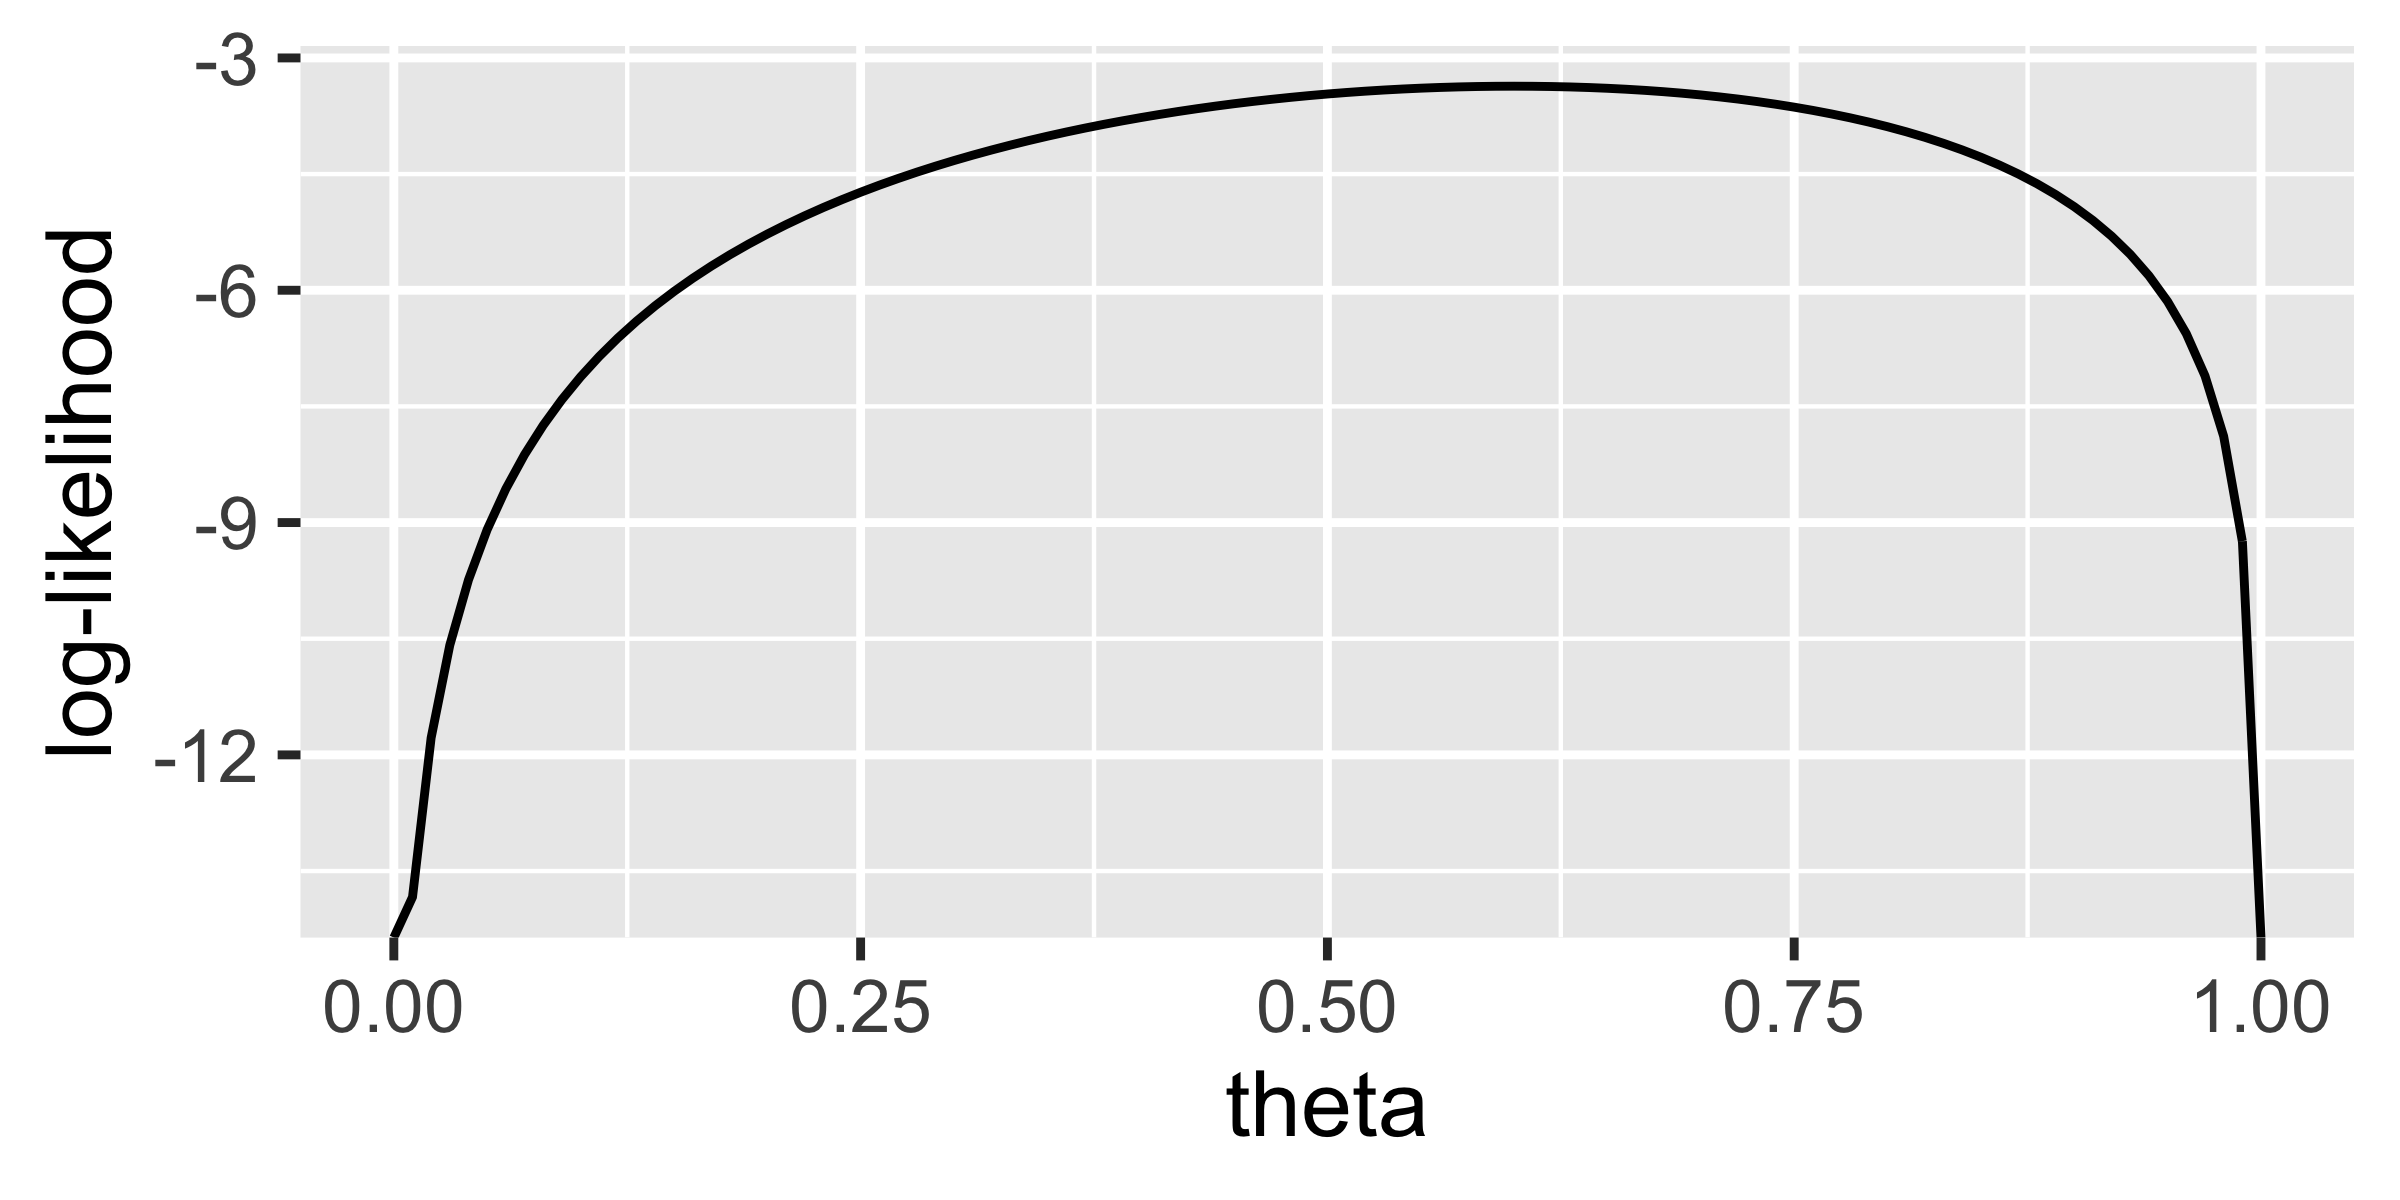
\includegraphics[keepaspectratio,width=6cm]{images/text24/Rplot24_02.png}
    \caption{「表，表，裏，裏，表」と出たコインのパラメータの関数について対数をとったもの。縦軸は対数尤度}
    \label{fig::24_02}
\end{figure}
\section{正規分布の尤度関数}
対数の話は計算上の問題なので知識として頭の片隅に置いておいてもらったらOKです。それよりも，関数の形をそのまま使ってパラメータを推定できる，ということをしっかり踏まえていただければと思います。この方法だと，不偏推定量を考えるとか，標準誤差を考えるといったことがなくなるので，もしかするとこちらの方が楽だな，と思われるかもしれません。注意しておきたいのは，これは「ある推定値が得られる確率」を考えているわけ
ではないことです(尤度は確率ではないので)。また，データに最もぴったり合うようにパラメータを定めた，という方法なだけで，そもそもデータに当て嵌める確率分布関数(=確率モデル)が間違っていたら，何の意味もないことに注意してください。コイントスの結果にはベルヌーイ分布(あるいは二項分布)を当て嵌めるのが正しく，他の分布--例えば正規分布--を考えると「答えは出るけど，そもそも全部間違ってる」というような話になります\footnote{適切な確率分布関数を選択できていないことなどを総称して，モデル誤設定問題と言います。}。とは言えここまで見てきたように，心理学の場合は，多くのデータに正規分布を仮定できます。私たちは正規分布という「仮定」，「モデル」をおいて現象を理解しようとしているんだ，ということを忘れないでください。

そう言えば，正規分布を使った最尤推定はどうなるんでしょうね。正規分布は平均$\mu$と標準偏差$\sigma$という2つのパラメータで調整されますから，この2つのパラメータが両方未知であるという連立方程式を解くことになります。

数値例を使って考えてみましょう。第\ref{chapter16}講で最初に考えた例，「ある小さな学校で身体測定をしたところ，3人の身長はそれぞれ，165cm,173cm,182cmだった」という話で考えてみたいと思います。話を単純にするために，母標準偏差は$\sigma=10$だとわかっていたとします。こうすることで，先ほどのベルヌーイ試行と同じで推定すべきパラメータはひとつ，$\mu$だけになりますから。

さて，これらのデータが何らかの正規分布，$N(\mu,10)$から得られたわけですが，仮に$\mu=160$だとすると，確率分布を描いて，実現値に対してどの程度「尤もらしいのか」を確率密度で計算できます(図\ref{fig::24_03})。各データ点に対応する確率密度は確率ではありませんが，どの程度生じやすいかを表している数字ではありますので，このまま利用できます。Rでの計算方法はもちろん，\texttt{dnorm(165,mean=160,sd=10)}とすれば良いですね！
\begin{figure}[ht]
    \centering
    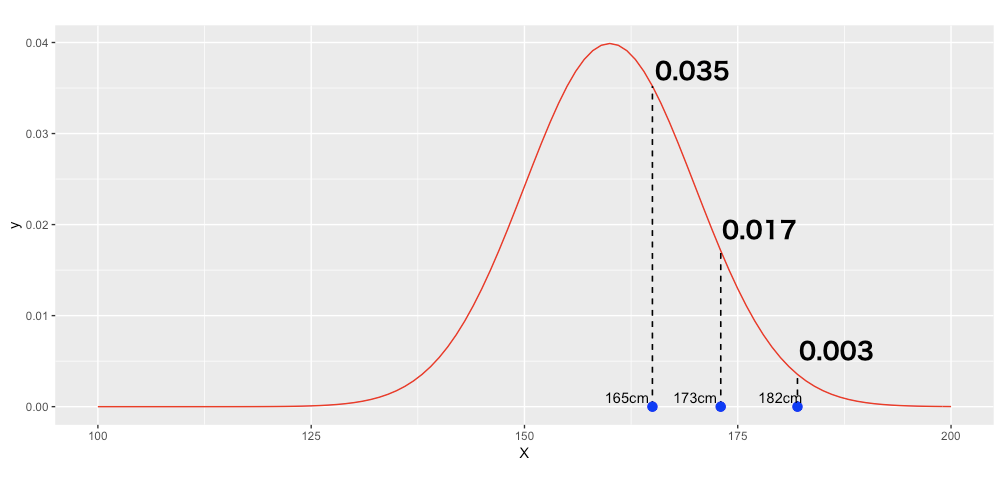
\includegraphics[keepaspectratio,width=12cm]{images/text24/slide24_01.png}
    \caption{}
    \label{fig::24_03}
\end{figure}
さて，これら3つのデータは同じ母集団から独立に得られているわけです。独立に，というのはデータ間に特に関連がないことですので，この3つが同時に成立する確率は掛け算で表すことができます\footnote{コイントスの場合もこの同じ分布から独立して得られている，という仮定がありました。同じコインですから同じ確率分布を仮定でき，独立というのは前の試行が次の試行に影響を与えない，という意味です。コイントスした時にコインが歪んでしまった(違う$\theta$になった)，というようなことは考えていませんから，毎回確率$\theta$で繰り返した時に，掛け合わせることができたのです。ちなみにこの仮定のことを独立同分布independently and identically distributedといい，i.i.dと略記されることがあります。}。これを計算すると，
$$ 0.035 \times 0.017 \times 0.003 = 0.0000002140286$$
になります。このようにとても小さい数字になりますので，対数をとって
$$ \log 0.035 +\log 0.017 +\log 0.003 = -13.05457$$
とした方がいいかもしれません。ほかに，$\mu=170$ならどうか，$\mu=190$ならどうか，といろいろ試すことができますが，要するにこの数字(尤度)は$\mu$の関数になっているわけです。そこで，横軸に$\mu$をとり，縦軸に尤度をとってグラフを書いてみますと，図\ref{fig::24_04}のようになります。
\begin{figure}[ht]
    \centering
    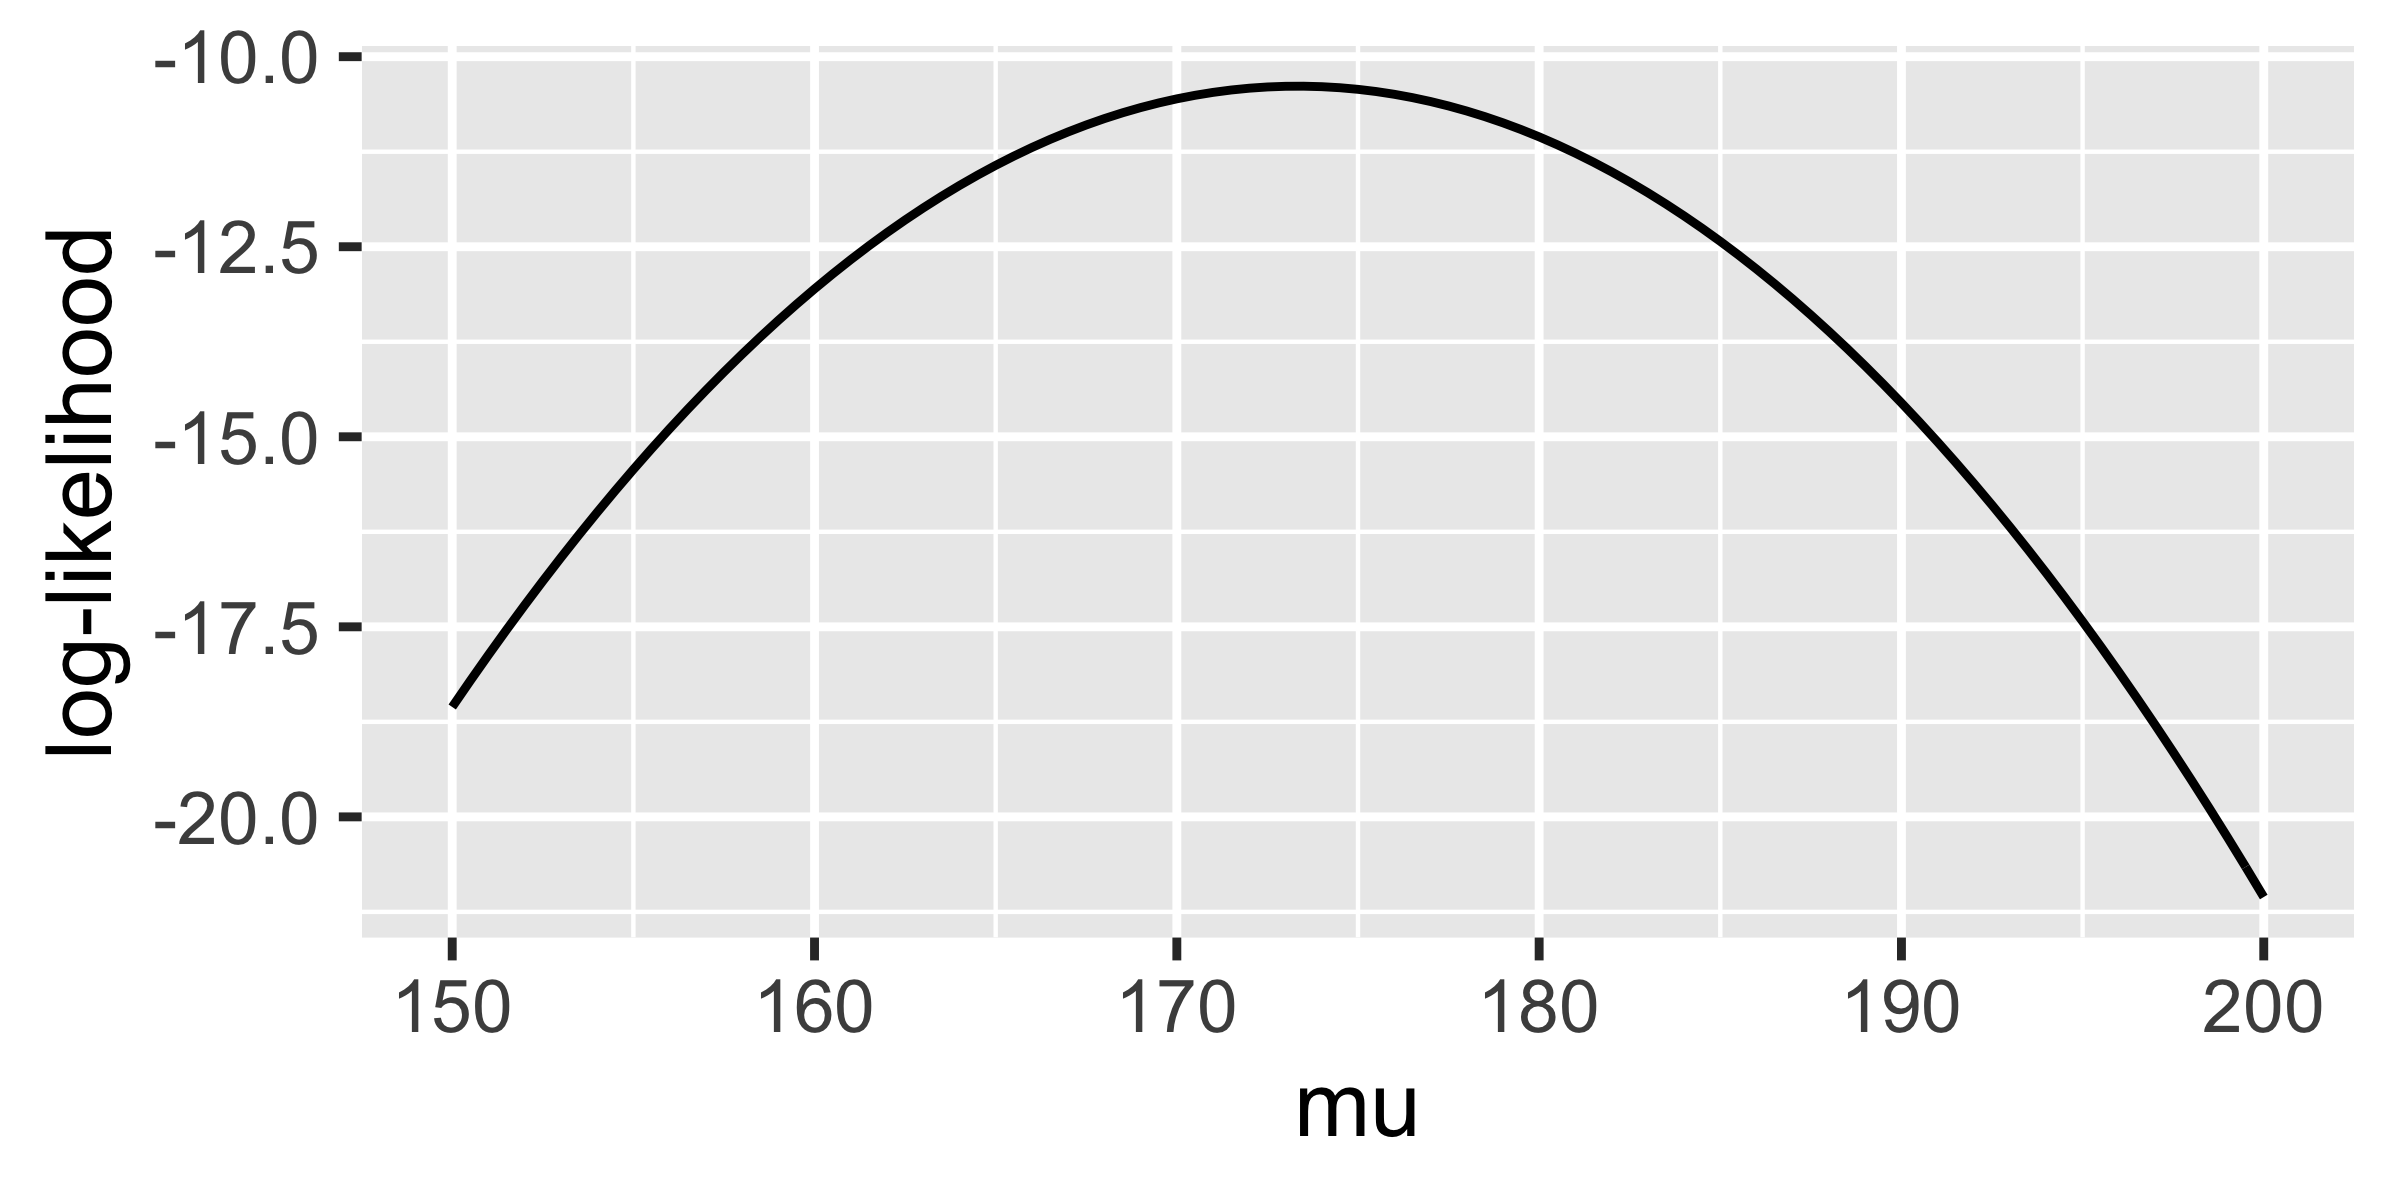
\includegraphics[keepaspectratio,width=12cm]{images/text24/Rplot24_03.png}
    \caption{正規分布の尤度を求める}
    \label{fig::24_04}
\end{figure}
このようにしてみると，確かに170を少し超えたあたりにピークがありそうです。ちなみにその最尤推定値は173.3であり，データの平均値と同じになります。

標本平均と同じじゃないか，と思うかもしれませんが，推定方法が違うだけで同じ母集団の推定方法なので，むしろ答えが一致してよかったね，と思ってください。ともかく，このように正規分布でも最尤推定はできます。が，今回は母標準偏差がわかっている($\sigma=10$)という仮定の下で計算したのでした。本来はこちらも推定しなければなりません。つまり，平均$\mu$と標準偏差$\sigma$2つの関数になるのです。

この2つの関数のグラフを書いたのが図\ref{fig::24_05}です。2つの変数で1つの対数尤度が決まるので，3次元プロットになりますし，2変数の微分方程式を解くことになるので数学的には少し面倒になりますが，同様に推定できることがわかります。最尤推定の結果は，標本平均と標本標準偏差の値と一致します\footnote{不偏分散の平方根($N-1$で割った方)じゃないのか，と思われるかもしれませんが，最尤推定による母SDの推定値は標本SDに一致します。}。
\begin{figure}[ht]
    \centering
    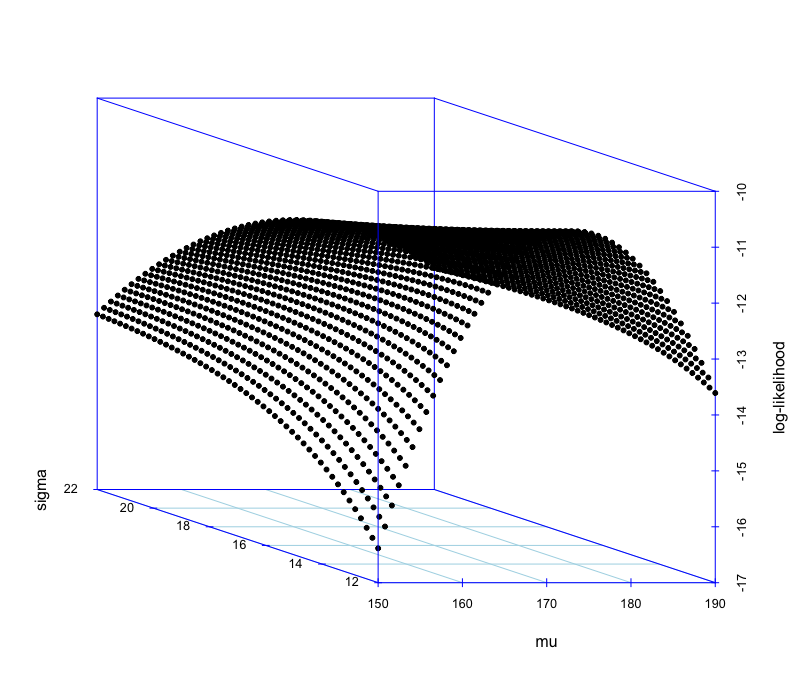
\includegraphics[keepaspectratio,width=12cm]{images/text24/Rplot24_04.png}
    \caption{平均と標準偏差による2変数関数としての正規分布の対数尤度}
    \label{fig::24_05}
\end{figure}

\section{ベイズの定理}
ここまで尤度を使った推定方法について説明してきました。モーメント法と最尤法，いずれも同じ答えが出るのですがその考え方が違うというところを確認してきましたね。ここでは最後に，もう1つの推定法であるベイズ法について解説します。そのためには，ベイズ法の根本的な法則について知っておいた方が良いので，少し回りくどいかもしれませんが，まずはそこから説明していきましょう\footnote{目的を先に教えてくれないとやだよ，という人のために一言で目的だけ言っておきます。ベイズ法は最尤法と同じく確率モデルを使うのですが，尤度が「確率じゃない」という妙な性質があったのに対し，ベイズ法は答えを確率で出します。尤度を確率にするための仕掛けがこれから始まるのです。}。
\subsection{ベイズの定理とは}
ベイズというのは人の名前で，トーマス・ベイズ（Thomas Bayes、1702年 - 1761年4月17日）はイギリスの長老派の牧師であり数学者でもある人です。この人の考えた「逆確率の法則」から端を発した推定法が，21世紀の現代においてとても重要なものになってきています。ベイズ牧師の考えついた法則は非常に単純なもので，簡単に書くと次のような式で表現できます。
$$ P(A|B) = \frac{P(B|A)P(A)}{P(B)}$$


例えば，ある学校の生徒数は男子が40人，女子が60人だったとします。そこからランダムに一人を選び出した時，それが男子である確率はどれぐらいでしょうか？この確率を$P(\mbox{男子})$とすると，
$$P(\mbox{男子})=\frac{40}{(100)}=0.4$$
であることはすぐにわかりますね。

では次に\keyterm{同時確率}という考え方を導入しましょう。これは先ほどの学校について，表\ref{tbl::24_02}のように学年情報を追加した例を使って説明します。


\begin{table}[ht]
    \centering
    \caption{ある学校の学年と性別のデータ} 
    \begin{tabular}{rrrrr}
      \hline
      & 1年 & 2年 & 3年 & 合計 \\
    \hline
    男子 & 15 & 12 & 13 & 40\\
    女子 & 22 & 20 & 18 & 60\\\hline
    合計 & 37 & 32 & 31 & 100\\\hline
    \end{tabular}
      \label{tbl::24_02}
\end{table}

ここでランダムに一人を選び出した時，それが「3年男子」である確率はどれぐらいでしょうか？これは「学年は3」かつ「性別は男」なので，学年と性別の両方の条件が入った同時確率といい，$P(\mbox{学年},\mbox{性別})$と書きます。これは表から，次のように計算できますね。
$$ P(\mbox{学年;3},\mbox{性別;男})= \frac{13}{100}=0.13$$

次に用語として\keyterm{周辺確率}というのを考えます。これはある分割に関して全て足し上げたもの，というものですが，要するに表\ref{tbl::24_02}の合計欄のことです。例えば「男子生徒についての周辺確率」は，男子生徒が学年によって3つに分割されていますが，これを全て足し上げるので，1年男子+2年男子+3年男子で求まるものです。なんてことはないですね。

では次のステップ。今度は\keyterm{条件つき確率}というのを導入します。無作為に学生を選び出す時，「選ばれたのが女子である」ということが先にわかったとします\footnote{例えば名前とか容易に類推できた，といったようなシーンです。}。その時，その生徒が2年生である確率はどれくらいでしょうか？この問いを「女子という条件がついた上での確率」という意味で，条件つき確率といい，表現としては$P(\mbox{2年生}|\mbox{女子})$と書きます。2つの分割を縦棒で区切り，条件の方が後ろに書きます。「女子という条件が与えられた上での二年生の確率は」というように読んだりします。

ちょっと状況はややこしくなりましたが，確率の計算そのものはそれほど難しくありませんね。女子である，というのが決まっているので，分母が変わるだけなのです。つまり，
$$P(\mbox{2年生}|\mbox{女子})=\frac{20}{60}=0.333...$$
となります。

条件つき確率の計算は分母が変わったと思えばいいのですね。この条件つき確率は，同時確率を周辺確率で割っても計算できます。すなわち，
$$ P(\mbox{2年生}|\mbox{女子}) = \frac{P(\mbox{2年生},\mbox{女子})}{P(\mbox{女子})}=\frac{0.2}{0.6}=0.333...$$

さて，これで用語の準備は終了です。ここから式の展開が面白くなってきます。記号で表現するために，性別の変数をAとし，$A_1=$男子，$A_2=$女子，学年の変数をBとして$B_1=$1年生，$B_2=$2年生，$B_3=$3年生としましょう。

あらためて，条件付き確率は同時確率を周辺確率で割ったもの，でしたね。つまり，
$$ P(B_j | A_i) = \frac{P(B_j,A_i)}{P(A_i)}$$
ここで右辺の分母を両辺にかけて，
$$ P(A_i)P(B_j|A_i) = P(B_j,A_i)$$
とします。これはA,Bが何であるかにかかわらず，一般的に成立します。たとえば$P(A_i|B_j)$と記号をひっくり返しても，
$$ P(A_i|B_j) = \frac{P(A_i,B_j)}{P(B_j)}$$
より
$$P(B_j)P(A_i|B_j) = P(A_i,B_j)$$
としても構いませんね。


ところで，「2年の男子」と「男子の2年」というのは同じ意味です。つまり，
$$P(B_j,A_i) = P(A_i, B_j)$$
ですから，上の式をつなぎ合わせて
$$P(A_i)P(B_j|A_i) = P(B_j)P(A_i|B_j)$$
とできます。ここで両辺を$P(B_j)$で割って清書すると，
$$ P(A_i | B_j )=\frac{P(B_j|A_i)P(A_i)}{P(B_j)}$$
が得られます。やったね！ベイズの定理が導出できました。


さて，これの何がすごいのでしょう？
\subsection{ベイズの定理の意味}
実は，\underline{左辺と右辺の中にある条件つき確率の中身がひっくり返っている}のがすごいんです。

凄さがピンとこないかもしれませんね。2年生だとか女子だとかだと，面白味がわからないかもしれませんので，別の言葉で考えてみましょうか。

コロナウイルスに感染しているかどうかは，PCR検査で明らかになりますが，これらの検査の結果というのも確率的な要素があるのはご存知でしょうか。本当は感染していないのに，検査では陽性になってしまう，ということがゼロではありません。こういうのを偽陽性といいます。逆に感染しているのに，検査で検出できずに陰性になる，偽陰性ということもあります。いずれも確率的な話です。

コロナに感染している$\to$検査で陽性になる，というのが因果関係ですが，我々は実際には検査で陽性である$\to$コロナに感染しているかもしれない，というように推論します。これを今日学んだ確率の言葉で書いてみましょう。

感染している状態で，陽性反応が出るというのは条件つき確率として表現できますね。$P(\mbox{陽性}|\mbox{感染})$，というわけです。さてここに，そもそもの感染率というのが別途見積もれたとします。$P(\mbox{感染})$ですね。さらにもうひとつ。感染しているかどうかに関係なく，陽性であるという結果だけ取り上げて$P(\mbox{陽性})$を考えることもできます。これが揃うと，先ほどの定理を使って
$$ \frac{P(\mbox{陽性}|\mbox{感染})P(\mbox{感染})}{P(\mbox{陽性})} = P(\mbox{感染}|\mbox{陽性})$$
を計算できます。つまり陽性になったという結果から，本当にかかっているかどうかの確率を計算できるのです。

多くの場合，検査で陽性だったら「もうだめだー」と思ってしまいがちです。これは陽性であると確実に検出できる，偽陽性がゼロの検査であれば正しい判断です。が，実際には確率的に判断すべき問題です。具体的に数字を例にして考えてみましょう。

\begin{itemize}
    \item 40歳の女性が乳がんにかかる確率は1\%です。
    \item 乳がんである人が乳房X線検査で陽性と出る確率は90\%です。
    \item 本当は乳がんでなくても，検査で陽性と出る確率は8\%にすぎません。
    \item あなたが40歳の女性で検査結果が陽性だったとしたら，あなたが乳がんである確率はどれぐらいでしょうか。
\end{itemize}
これは先ほどの公式に当てはめて考えると，
$$\frac{0.9\times0.01}{0.9\times0.01+0.08\times0.99}=0.102 $$

となり，10\%ちょっとだということになります\footnote{おっと，計算についていけないぞ！と思った人。大丈夫です，いい方法があります。確率の計算は小数点を含みますし相対的な度数なのでわかりにくいですから，絶対的な度数に戻して考えればいいのです。例えば10000人の世界だとして考えると，乳がんの人は1\%=100人です。乳がんでない人は9900人です。陽性になる人は乳がんで陽性反応が出るひと($100\times0.9=90$)と乳がんじゃないのに陽性反応が出る人($9900\times0.08=792$)の和で，882人です。陽性反応が出た人の中で本当に乳がんであるひとは，$90/882=0.102$となります。}。ずいぶんと印象が変わりますよね。PCR検査を複数回行うのは，これと同じような背景があるからです。

話を本題に戻しましょう。我々は心理学の研究の話をしているはずなのですから。

大事なのは，不確かな状況においては我々は確率的にしか判断をできず，ベイズの定理では条件の向きをひっくり返して計算できる，という点です。原因が結果を引き起こす確率が知りたい時に，結果を手にすることで，原因がどれほどあり得たかを考えることができる。それがベイズの定理のポイントなのです。

ベイズの定理の左辺には$P(A|B)$があり，右辺は分子に$P(B|A)$を含んでいます。$P(A)$(分子の2つ目の項目)や$P(B)$(分母)のことは一旦忘れてくれてもいいですし，
$$ P(A|B) = P(B|A) \times \frac{P(A)}{P(B)}$$
と考えて，$P(A|B)$が$P(B|A)$の関数である，と読み取ってくれても構いません。
ここでAを「心のモデル」，Bを「データ」と考えてみてください。

私たちは心の仕組みを考える時に，モデルをたてます。「あの人が$\diamond\diamond\diamond\diamond$な行動をとったのは，心の状態が$\dagger\dagger\dagger\dagger$だったからではないか」というのは心というモデルを立てて考えるということなのでした。心の状態が$\dagger\dagger\dagger\dagger$であれば，人は$\diamond\diamond\diamond\diamond$な行動をとるであろう，というのが研究者の仮説，モデルなのです。つまり，$P(\mbox{データ}|\mbox{モデル})$が心理学でやっていることなのです。

ところが実際には，手に入れることができるのはデータだけです。心がどうなっているかはわかりませんが，人が$\diamond\diamond\diamond\diamond$な行動をとった，という事実だけがそこにあるのです。この事実を使って，我々のモデルがどれぐらい正しいのか。あるいはモデルのパラメータはどうなっているのか，を検証したいわけです。つまり，研究の営みとは$P(\mbox{モデル}|\mbox{データ})$であり，データを所与(条件)としたときの，モデルの確率を考えることなのです。データをとってモデルを検証するという営みが成り立つ根拠を，ベイズの定理が示してくれていると言えるかもしれません\footnote{注意が必要なのは，モデルの正しい確率が検証されるわけではないところです。モデルを仮定すると，そのモデルから考えられる結果の確率がこれぐらいになる，という推論をしているのであり，モデルがそもそも前提されていますから，モデルが間違っていれば(例えばコイントスという現象に正規分布を当てはめて考えるとか)，その推論は全然正しいものではありません。}。

ベイズの定理を使ってパラメータを推論する時に，この定理が根本にあるということの意味が伝わりましたでしょうか。


\section{課題}

\end{document}
